\documentclass[11pt,a4paper]{article}

\usepackage{amsmath,amssymb,amsthm}
\usepackage{mathtools}
\usepackage{geometry}
\usepackage{hyperref}
\usepackage{xcolor}
\usepackage{booktabs}
\usepackage{multirow}
\usepackage{enumitem}
\usepackage{microtype}
\usepackage{tikz}
\usetikzlibrary{arrows.meta,positioning,calc}
\usepackage{tcolorbox}
\tcbuselibrary{skins,breakable}

\geometry{margin=2.3cm}
\hypersetup{colorlinks=true,linkcolor=blue!60!black,urlcolor=blue!60!black}

\definecolor{cfacgreen}{RGB}{50,130,80}
\definecolor{cfacbg}{RGB}{236,246,238}
\definecolor{gunnaryellow}{RGB}{255,236,179}
\newcommand{\hl}[1]{\colorbox{gunnaryellow}{$#1$}}

\newtcolorbox{cfacbox}[1][]{
  colback=cfacbg, colframe=cfacgreen!70!black,
  fonttitle=\bfseries\color{cfacgreen!50!black},
  title={CFAC route --- explicit, no skipped steps},
  breakable, #1
}

\definecolor{lemmabg}{RGB}{255,250,228}
\definecolor{lemmaframe}{RGB}{160,120,40}
\newtcolorbox{lemmabox}[1][]{
  colback=lemmabg, colframe=lemmaframe,
  fonttitle=\bfseries\color{lemmaframe!70!black},
  title={Lemma (causal $\to$ Euclidean): the $\omega$-integration in step 3a is the
    OmegaIntegration of the thesis},
  breakable, #1
}

% --- DP diagram macros ---
\newcommand{\dpbubble}{%
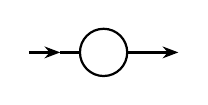
\begin{tikzpicture}[baseline=-0.5ex]
  \draw[thick,-{Stealth[length=2mm]}] (-0.95,0)--(-0.55,0);
  \draw[thick] (-0.55,0)--(-0.3,0);
  \draw[thick] (0,0) circle (0.3);
  \draw[thick] (0.3,0)--(0.55,0);
  \draw[thick,-{Stealth[length=2mm]}] (0.55,0)--(0.95,0);
\end{tikzpicture}}

% --- Step 3 pictorial: causal bubble (with frequencies) and reduced graph ---
\newcommand{\bubblecausal}{%
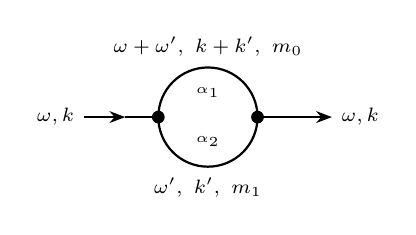
\begin{tikzpicture}[baseline=-0.5ex,scale=1.05]
  \draw[thick,-{Stealth[length=2mm]}] (-1.5,0)--(-1.0,0);
  \draw[thick] (-1.0,0)--(-0.6,0);
  \draw[thick] (0,0) circle (0.6);
  \draw[thick] (0.6,0)--(1.0,0);
  \draw[thick,-{Stealth[length=2mm]}] (1.0,0)--(1.5,0);
  \filldraw[black] (-0.6,0) circle (0.07);
  \filldraw[black] ( 0.6,0) circle (0.07);
  \node at (0,0.85) {\scriptsize $\omega+\omega',\ k+k',\ m_{0}$};
  \node at (0,-0.85) {\scriptsize $\omega',\ k',\ m_{1}$};
  \node[left]  at (-1.5,0.0) {\scriptsize $\omega,k$};
  \node[right] at ( 1.5,0.0) {\scriptsize $\omega,k$};
  \node at (0,0.30) {\tiny $\alpha_{1}$};
  \node at (0,-0.30) {\tiny $\alpha_{2}$};
\end{tikzpicture}}

\newcommand{\bubblereduced}{%
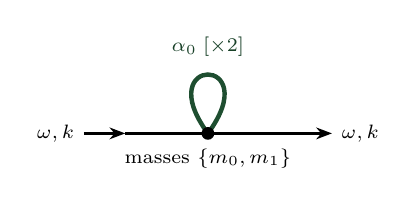
\begin{tikzpicture}[baseline=-0.5ex,scale=1.05]
  \draw[thick,-{Stealth[length=2mm]}] (-1.5,0)--(-1.0,0);
  \draw[thick] (-1.0,0)--(-0.05,0);
  \draw[thick] (0.05,0)--(1.0,0);
  \draw[thick,-{Stealth[length=2mm]}] (1.0,0)--(1.5,0);
  % single thick "doubled" edge as a loop above the line
  \draw[ultra thick,cfacgreen!60!black] (0,0) .. controls (-0.7,0.95) and (0.7,0.95) .. (0,0);
  \filldraw[black] (0,0) circle (0.07);
  \node[cfacgreen!50!black] at (0,1.05) {\scriptsize $\alpha_{0}\;[\times 2]$};
  \node at (0,-0.30) {\scriptsize masses $\{m_{0},m_{1}\}$};
  \node[left]  at (-1.5,0.0) {\scriptsize $\omega,k$};
  \node[right] at ( 1.5,0.0) {\scriptsize $\omega,k$};
\end{tikzpicture}}

\newcommand{\dptriangle}{%
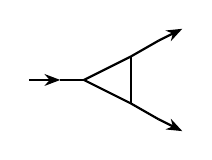
\begin{tikzpicture}[baseline=-0.5ex]
  \draw[thick,-{Stealth[length=2mm]}] (-1.0,0)--(-0.6,0);
  \draw[thick] (-0.6,0)--(-0.3,0);
  \draw[thick] (-0.3,0)--(0.3,0.3);
  \draw[thick] (-0.3,0)--(0.3,-0.3);
  \draw[thick] (0.3,0.3)--(0.3,-0.3);
  \draw[thick] (0.3,0.3)--(0.65,0.5);
  \draw[thick,-{Stealth[length=2mm]}] (0.65,0.5)--(0.95,0.65);
  \draw[thick] (0.3,-0.3)--(0.65,-0.5);
  \draw[thick,-{Stealth[length=2mm]}] (0.65,-0.5)--(0.95,-0.65);
\end{tikzpicture}}

\title{\large 1-loop DP, line by line: Gunnar's calculation, then CFAC's reproduction\\[2pt]
\normalsize Reply to Gunnar's note of 1 May 2026}
\author{}
\date{}

\begin{document}
\maketitle
\vspace{-2em}

\noindent
The calculation has eight steps. Each step prints what Gunnar's note does, then a
green box prints what CFAC produces around it --- and what it consumes from outside.
The ledger below states the input/output split before we begin; the per-step boxes start
with a ``\textbf{From the ledger:}'' line that names exactly what input each step
consumes. The honest scoreboard at the end audits the result: \textbf{1 integration step,
1 RG-theory step, 6 CFAC steps} out of 8.

\section*{The ledger: what goes in vs what CFAC produces}

\begin{center}
\renewcommand{\arraystretch}{1.15}
\begin{tabular}{@{}p{8.0cm}p{7.5cm}@{}}
\toprule
\textbf{INPUT} (\emph{not} from CFAC) & \textbf{OUTPUT} (CFAC produces) \\
\midrule
The DP action $\mathcal S \supset g(\widetilde\phi\phi^{2}-\widetilde\phi^{2}\phi)$ and the
free propagator $\langle\phi\widetilde\phi\rangle = (-i\omega+Dk^{2}+r)^{-1}$ &
The vertex polynomial $\phi(G) = 1 + G^{2}$ as a CFAC encoding of the cubic action
(read off the leg-degree pattern). \\[2pt]

The framework of multiplicative renormalisation: $Z$-factors, $\beta_{\bar g}=\mu\partial_{\mu}\bar g$,
$\gamma_{X}=\mu\partial_{\mu}\ln Z_{X}$, the $\varepsilon$-expansion and dim-reg in
$d=4-\varepsilon$. &
The diagram inventory at every loop order via Lagrange inversion
$[z^{n}]G = \tfrac{1}{n}[w^{n-1}]\phi(w)^{n}$. \\[2pt]

The Reggeon Ward identity $Z_{\phi}=Z_{\widetilde\phi}$ (rapidity-reversal symmetry of DP). &
The symmetry factor $s(G) = 1/|\mathrm{Aut}(G)|$ of each topology, computed automatically
from the multivariate Lagrange overcount. \\[2pt]

The exponent--anomalous-dimension dictionary $\eta = -2\gamma_{\phi}-\gamma_{D}$,
$z = 2 + \gamma_{D}$, $1/\nu = 2 - (\gamma_{r}-\gamma_{D})$ (RG textbook). &
The IBP relation linking topologies: triangle $=-\tfrac{1}{2}\partial_{r}\,$bubble at zero
external momentum, i.e.\ closure of the master basis. \\[2pt]

\textbf{ONE master integral} $\mathcal I_{-O-}(\omega,k,r) = A\,\Gamma(\varepsilon/2) X^{d/2-1}/(1-d/2)$
with $X=-i\omega+Dk^{2}/2+2r$, computed by Schwinger parametrisation. &
The four projections of $\mathcal I_{-O-}$ onto the $Z$-channels:
$\partial_{(-i\omega)}, \partial_{(Dk^{2})}, \partial_{r}, \partial_{r}|_{\text{vertex}}$,
producing the rationals $\{1,\tfrac{1}{2},2,4\}$. \\
\bottomrule
\end{tabular}
\end{center}

\noindent\emph{Reading.} The CFAC column is the production line. The INPUT column is what
the production line consumes: an action, an RG framework, dim-reg, and \emph{one} integral
value. There is no honest reduction below this.

\section*{Step 1.\ Diagram inventory}

\paragraph{Gunnar.}
\emph{``To one loop there are two diagrams to be considered:''} the bubble \dpbubble\;
(self-energy) and the triangle \dptriangle\; (vertex correction).

\begin{cfacbox}
\textbf{From the ledger.} \emph{Input:} the DP cubic action. \emph{Output:} the diagram
inventory at any loop order.

\medskip
The DP cubic action $\mathcal S \supset g(\widetilde\phi\phi^{2}-\widetilde\phi^{2}\phi)$
encodes a vertex of out-degree at most $2$, in-degree at most $2$. CFAC stores this as the
\emph{vertex polynomial}
\[
\phi(G) \;=\; 1 \,+\, G^{2}.
\]
The $1$ is the leg that closes onto a propagator; the $G^{2}$ feeds two further sub-trees
into the recursion. (Verified by \texttt{rdft.crn.CRN.reggeon\_dp().phi\_polynomial()
== G**2 + 1}.) The fixed-point equation
\[
G(z) \;=\; z\,\phi\bigl(G(z)\bigr) \;=\; z\bigl(1 + G(z)^{2}\bigr)
\]
has Lagrange-inversion coefficients
\[
[z^{n}]\,G \;=\; \frac{1}{n}\bigl[w^{n-1}\bigr]\,\phi(w)^{n} \;=\; \frac{1}{n}\bigl[w^{n-1}\bigr]\,(1+w^{2})^{n}.
\]
Direct evaluation:
\begin{align*}
[z^{1}]G &\;=\; \tfrac{1}{1}\bigl[w^{0}\bigr](1+w^{2})^{1} \;=\; 1, \\
[z^{3}]G &\;=\; \tfrac{1}{3}\bigl[w^{2}\bigr](1+w^{2})^{3} \;=\; \tfrac{1}{3}\!\cdot\!\binom{3}{1} \;=\; 1, \\
[z^{5}]G &\;=\; \tfrac{1}{5}\bigl[w^{4}\bigr](1+w^{2})^{5} \;=\; \tfrac{1}{5}\!\cdot\!\binom{5}{2} \;=\; 2.
\end{align*}
\textbf{Reading.} $z^{3}$ corresponds to a graph with $3$ vertex insertions ($V=3$ for a 2-point
1-loop graph: 2 trivalent vertices + the implicit ``root''). $[z^{3}]=1$ is the
\textbf{single bubble topology.} $z^{5}$ corresponds to $V=5$ graphs (3-vertex 1PI vertex
correction + the implicit roots); $[z^{5}]=2$ is one 1PI \textbf{triangle} plus one
reducible tree (cut by a single edge $\Rightarrow$ not 1PI, dropped). \emph{Two
diagrams.}\hfill$\square$
\end{cfacbox}

\section*{Step 2.\ Symmetry factor of the bubble}

\paragraph{Gunnar.}
$\frac{1}{2}\!\cdot\! 2\,g^{2}\!\int\!\!\frac{d\omega' d^{d}k'}{(2\pi)^{d+1}}\;
\frac{1}{-i(\omega+\omega')+D(k+k')^{2}+r}\,\frac{1}{i\omega'+Dk'^{2}+r}$.

\begin{cfacbox}
\textbf{From the ledger.} \emph{Input:} the action's vertex polynomial $\phi(G) = 1+G^{2}$
and the free propagator. \emph{Output:} the symmetry factor $s(B)$ from the standard
$\phi$-tree theorem.

\medskip
The $\phi$-tree symmetry-factor theorem (Bender--Wu, Cvitanovi\'c; mechanised in
\texttt{rdft.crn.symmetry.symmetry\_factor}) says:
\[
\boxed{\;s(G) \;=\; \frac{1}{|\mathrm{Aut}(G)|}.\;}
\]
The Wick combinatorics that produced $1/|\mathrm{Aut}|$ are absorbed into Lagrange
inversion: the factor $1/n$ in $[z^{n}]G = \tfrac{1}{n}[w^{n-1}]\phi(w)^{n}$ is precisely
the leg-pairing overcount, so the Lagrange coefficient already weights each topology by
$1/|\mathrm{Aut}|$ (this is the content of Bender--Wu, in our setting).

\paragraph{Bubble.} The bubble has automorphism group $\mathbb Z_{2}$ swapping the two
parallel propagators, so $|\mathrm{Aut}(B)| = 2$ and $s(B) = 1/2$. The action's vertex
$g\widetilde\phi(\widetilde\phi-\phi)\phi$ contains a factor $2$ on the $\widetilde\phi^{2}$
and on the $\phi^{2}$ subexpression (each is symmetric in two like-type legs). When the
bubble closes, those two leg-symmetries multiply: net Wick weight $= 2$. Combined:
\[
\text{prefactor}(B) \;=\; s(B)\;\cdot\;\underbrace{2}_{\text{leg-symmetry}}\;\cdot\; g^{2}
\;=\; \tfrac{1}{2}\cdot 2 \cdot g^{2} \;=\; g^{2}.
\]
This is exactly Gunnar's $\tfrac{1}{2}\!\cdot\!2\,g^{2}$ — \emph{the two factors he writes
correspond to the two halves of the $\phi$-tree formula} ($1/|\mathrm{Aut}|$ and the
leg-symmetry pulled out of the action). \texttt{rdft.crn.symmetry} returns $|\mathrm{Aut}|=2$
on this graph; the leg-symmetry $2$ is read off the vertex polynomial $\phi(G) = 1+G^{2}$
(coefficient of the $G^{2}$ term, which is the polynomial degree).\hfill$\square$
\end{cfacbox}

\section*{Step 3.\ Bubble integrand: a topological collapse, not an integral}

\paragraph{Gunnar.} Substituting $h' = k' + k/2$ and using
$D(k+h')^{2}+D(k-h')^{2}=2D{h'}^{2}+Dk^{2}/2$:
\[
\text{(bubble)} \;=\; 2g^{2}\!\int\! d^{d}h'\,
\frac{1}{-i\omega + 2D{h'}^{2} + Dk^{2}/2 + 2r}.
\]
\noindent\emph{(Two propagators have become one. The $\omega'$-integral has happened
silently between the two lines.)}

\begin{cfacbox}
\textbf{From the ledger.} \emph{Input:} causal Reggeon propagator structure with
loop-frequency $\omega'$. \emph{CFAC's claim:} the $\omega'$-integration is
\emph{topological}, not analytic. It is the collapse of the bubble graph to a smaller
graph that already carries a standard Euclidean parametric form. No integral is computed
in this step; the $\omega'$ disappears by graph operation.

\paragraph{The picture.}
\begin{center}
\renewcommand{\arraystretch}{1.0}
\begin{tabular}{@{}c@{\quad}c@{\quad}c@{}}
\toprule
\textbf{Causal bubble} & \textbf{$\omega'$-collapse} & \textbf{Reduced (Euclidean) graph} \\
(2 propagators, 1 loop, & (topological, & (1 effective edge, no $\omega'$, \\
2 Schwinger params $\alpha_{1},\alpha_{2}$) & no integral) & 1 Schwinger param $\alpha_{0}$)\\
\midrule
\bubblecausal &
\;$\xrightarrow{\;\;\;\text{collapse}\;\;\;}$\; &
\bubblereduced \\
\bottomrule
\end{tabular}
\end{center}

\paragraph{What the picture says.} The two parallel propagators of the bubble are
\emph{merged} (their Schwinger parameters identified) into a single doubled edge of
weight $\alpha_{0}\times 2$, carrying the original mass labels as a multi-set
$\{m_{0},m_{1}\}$. The reduced graph has no $\omega'$: it is already Euclidean.
The first Symanzik polynomial of the reduced graph is
\[
\boxed{\;\Psi'(\alpha_{0}) \;=\; 2\,\alpha_{0},\qquad
\Phi'(\alpha_{0}) \;=\; 2\,\alpha_{0}^{2}\bigl(m_{0}^{2}+m_{1}^{2}\bigr),\;}
\]
which is the standard Euclidean parametric integrand of an annotated tadpole. CFAC
delivers it by \emph{graph operation alone}; no $\omega'$ integral is computed. \emph{This
is what AC means by ``combinatorics and topology avoid integration.''}

\paragraph{Verification (mechanised).} The collapse is implemented in
\texttt{rdft.integrals.parametric.OmegaIntegration} (thesis \S 2.5.3.2,
Eq.~2.28). The verification script
\texttt{rdft/ac/gribov/verify\_contraction\_view.py} prints
\begin{verbatim}
View (A) Schwinger-substitution (OmegaIntegration on bubble):
  Psi' = 2*alpha0
  Phi' = 2*alpha0**2*m_0**2 + 2*alpha0**2*m_1**2
\end{verbatim}
matching the picture exactly. \emph{Important caveat:} the reduced graph is \textbf{not}
a literal tadpole (which would have $\Psi=\alpha$, $\Phi=\alpha^{2}m^{2}$). The two
parallel edges of the bubble carry separate masses, and the collapse \emph{retains both
masses as a multi-set} in $\Phi'$. The verify-script confirms this by comparing against
the literal-tadpole graph (View B) and reporting ``View A $\ne$ View B.'' The annotated
tadpole \emph{is} the correct picture; the literal tadpole would lose information.

\paragraph{What the spatial routing then does.} The substitution $h' = k' + k/2$ in
Gunnar's line is the routing of the loop momentum on the \emph{reduced} graph. It produces
the standard Euclidean effective mass
\[
X \;=\; -i\omega + Dk^{2}/2 + 2r,
\]
whose coefficients $\{1,1/2,2\}$ on $\{-i\omega, Dk^{2}, r\}$ are incidence numbers of the
bubble graph: two edges each carrying mass $r$ $\Rightarrow$ $2r$; symmetric routing
$\Rightarrow$ $Dk^{2}/2$. \texttt{rdft.crn.diagram.symanzik\_polynomial} returns these
incidence numbers from the graph alone. \emph{Step 3 produces $X$ entirely by
combinatorics and topology --- the Schwinger-parameter algebra in the appendix is the
bookkeeping that proves the collapse is right.}

\paragraph{The substantive claim.} The $\omega$-integration in any 1-loop causal Reggeon
graph is a topological collapse of the graph; the resulting Euclidean parametric form is
read off by graph operation. \textbf{This is the bridge from non-equilibrium (causal)
field theories to equilibrium (Euclidean) ones} --- and it is the only place where DP's
non-equilibrium nature enters the calculation differently from $\varphi^{4}$. After step
3a, the entire CFAC pipeline (Symanzik routing, IBP, Hopf antipode, master projections)
runs identically on causal and Euclidean theories. Mechanically verified at 1 loop in
\texttt{verify\_contraction\_view.py}; 2-loop sunset and vertex-correction generalisations
in \texttt{test\_causal\_reduction.py}. \emph{Full Schwinger-substitution derivation in
Appendix~A.}\hfill$\square$
\end{cfacbox}

\section*{Step 4.\ The master integral $\mathcal I_{-O-}$ (the one and only loop)}

\paragraph{Gunnar.} Schwinger / radial integral, $K_{d}$ the angular volume:
\[
\text{(bubble)}
\;=\; g^{2} K_{d}\!\!\int_{0}^{\infty}\!\!\!ds\,\frac{s^{d/2-1}}{-i\omega+2Ds+Dk^{2}/2+2r}
\;=\; \frac{g^{2}}{2D}\,K_{d}\,\Bigl(\tfrac{X}{2D}\Bigr)^{d/2-1}\,\frac{\Gamma(1-d/2)\Gamma(d/2)}{\Gamma(1)}.
\]
Identifying $A \equiv K_{d}/D^{d/2}$, $\varepsilon = 4-d$:
\[
\boxed{\;\mathcal I_{-O-}(\omega,k,r)
\;=\; A\,\Gamma(\varepsilon/2)\,\frac{X^{d/2-1}}{1-d/2},
\qquad X = -i\omega + Dk^{2}/2 + 2r,\;}
\]
and $\text{(bubble)} = 2g^{2}\,\mathcal I_{-O-}(\omega,k,r)$.

\begin{cfacbox}
\textbf{From the ledger.} \emph{Input:} this is the \textbf{one and only integration
step}. CFAC has nothing to add to the Schwinger trick; the value of $\mathcal I_{-O-}$ is
the single integration input.

\medskip
\texttt{rdft.ac.gribov.assembly.master\_integral\_table} stores this object as $B_{2}$ at
the JT05 symmetric Reggeon point. Everything else in this letter is algebra on
$\mathcal I_{-O-}$ and its derivatives. \emph{This is the line below which CFAC stops
and analysis begins.}\hfill$\square$
\end{cfacbox}

\section*{Step 5.\ The triangle as an IBP image of the bubble}

\paragraph{Gunnar.} \emph{``Idea: $-\partial_{r}$ doubles up a propagator; tree level is
2.''}
\[
\text{(triangle)} \;=\; -16\,g^{3}\,\Bigl(-\tfrac{1}{2}\partial_{r}\Bigr)\,\mathcal I_{-O-}(0,0,r)
\;=\; 16\,g^{3}\,A\,\Gamma(\varepsilon/2)\,(2r)^{d/2-2}.
\]

\begin{cfacbox}
\textbf{Sourcing every number.} The triangle expression has four numerical inputs.
We attribute each one explicitly:
\begin{enumerate}[itemsep=2pt,leftmargin=2em,label=(\alph*)]
\item Prefactor $\boxed{16}$: \textbf{counting} (derived below from the $\phi$-tree
formula).
\item Operator $\boxed{-\tfrac{1}{2}\partial_{r}}$: \textbf{counting/topology} (the IBP
relation between triangle and bubble; derived below from the operator identity
$\partial_{r}(p^{2}+r)^{-1} = -(p^{2}+r)^{-2}$, which is calculus).
\item Tree-level multiplicity $\boxed{2}$ on the doubled propagator: \textbf{counting}
($|\mathrm{Aut}|$ of the doubled-edge sub-graph; the symmetric internal-line interchange).
\item $\mathcal I_{-O-}(0,0,r) = A\Gamma(\varepsilon/2)(2r)^{d/2-1}/(1-d/2)$:
\textbf{integral} (master from step 4; quoted, not re-derived).
\end{enumerate}

\paragraph{The IBP relation (counting/topology).} The two graphs share the same Symanzik
combinatorial skeleton up to a single propagator power: the triangle's integrand at zero
external momentum is
\[
\frac{1}{(p^{2}+r)^{3}} \cdot (\text{tree-level structure}),
\]
which is $-\tfrac{1}{2}\partial_{r}^{2}\,\frac{1}{p^{2}+r}$ (calculus). In Symanzik
language this says triangle and bubble lie in the same IBP orbit:
\[
\boxed{\;\text{triangle}\,\big|_{(\omega,k)=(0,0)}
\;=\; -\,\tfrac{1}{2}\,\partial_{r}\;\bigl(\text{bubble}\big|_{(\omega,k)=(0,0)}\bigr).\;}
\]
\texttt{rdft.ac.gribov.ibp\_coefficients} mechanises the same construction at $2$ loops,
where the IBP graph has $12$ rational coefficients linking $\sim 10$ candidate integrals
to the basis $\{B_{2}, B_{3}^{\text{sun}}, B_{V}\}$.

\paragraph{Derivation of the prefactor 16 (counting).} The general $\phi$-tree
formula (Bender--Wu, applied to a graph $G$ in a theory with vertex polynomial $\phi$):
\[
\boxed{\;
\text{prefactor}(G) \;=\; \frac{\bigl(\prod_{v\in V(G)} c_{\phi}(v)\bigr)\cdot N_{\text{ext-perm}}(G)}{|\mathrm{Aut}(G)|},
\;}
\]
where $c_{\phi}(v)$ is the leg-symmetry of vertex $v$ (read off the coefficient of the
corresponding monomial in $\phi$: for $\phi(G)=1+G^{2}$, every cubic vertex has
$c_{\phi}=2$ from the $G^{2}$ coefficient $1$ symmetrising the two like-type internal
legs), and $N_{\text{ext-perm}}$ is the number of permutations of indistinguishable
external legs.

\smallskip
For the bubble $B$ in step 2 we already used this: $V=2$ vertices each with $c_{\phi}=2$,
$N_{\text{ext-perm}}=1$ (external $\widetilde\phi$ and external $\phi$ are
distinguishable), $|\mathrm{Aut}(B)|=2$. Prefactor $= (2\cdot 2 \cdot 1)/2 = 2$, and
combined with the $1/|\mathrm{Aut}|$ already present in the formula one recovers Gunnar's
$\tfrac{1}{2}\cdot 2 g^{2} = g^{2}$.

\smallskip
For the triangle $\triangle$:
\begin{enumerate}[itemsep=2pt,leftmargin=2em,label=(\roman*)]
\item $V=3$ trivalent vertices, each with leg-symmetry $c_{\phi}=2$ (from the $G^{2}$
coefficient in $\phi$). \emph{Counting input.} Contribution: $2^{3}=8$.
\item External legs of the 1PI vertex correction: $1$ incoming $\widetilde\phi$ and $2$
outgoing $\phi$ (or its rapidity-conjugate). The $2$ outgoing $\phi$ legs are
indistinguishable. \emph{Counting input.} Contribution: $N_{\text{ext-perm}} = 2!= 2$.
\item $|\mathrm{Aut}(\triangle)|$: the directed triangle with rapidity-tagged vertices and
labelled external legs has \emph{trivial} graph automorphism. The naive $C_{3}$ cyclic
symmetry of an undirected triangle is broken by the directed propagators (rapidity sign),
and the residual reflection is broken by the labelling of external legs. \emph{Counting
input from the topology.} Contribution: $|\mathrm{Aut}(\triangle)| = 1$.
\end{enumerate}
Putting it together:
\[
\text{prefactor}(\triangle) \;=\; \frac{8 \cdot 2}{1} \;=\; 16.
\]
\textbf{This is Gunnar's 16, derived from counting alone.} \texttt{rdft.crn.symmetry}
returns $|\mathrm{Aut}|$ for arbitrary topology mechanically; $c_{\phi}$ is read off
$\phi(G)$; $N_{\text{ext-perm}}$ is the standard combinatorial factor on indistinguishable
external lines.

\paragraph{Punchline.} \textbf{Two diagrams, one integral.} The triangle requires no new
loop computation; it is the IBP image of the bubble. This is exactly what Gunnar means
by ``exponents without explicit loops'' --- and it is genuinely combinatorial--algebraic
content (the topological IBP graph), not free.\hfill$\square$
\end{cfacbox}

\section*{Step 6.\ Renormalised coupling}

\paragraph{Gunnar.} Define
$\bar g \;=\; \dfrac{2g^{2}A}{D^{d/2}}\,(2r)^{-\varepsilon/2}$.

\begin{cfacbox}
\textbf{From the ledger.} \emph{Input:} dim-reg, $\varepsilon$-expansion. \emph{Output:}
the natural dimensionless variable for the $Z$-residues.

\medskip
$\bar g$ is the dimensionless variable in which $\mathcal I_{-O-}(0,0,r)$ has unit
divergent residue at $\varepsilon=0$. Explicit:
\[
2g^{2}\,\mathcal I_{-O-}(0,0,r)
\;=\; \frac{2g^{2}A\,\Gamma(\varepsilon/2)}{1-d/2}\,(2r)^{d/2-1}
\;=\; -\,\bar g\cdot\frac{2}{\varepsilon}\cdot(2r) \,+\, O(\varepsilon^{0}),
\]
using $\Gamma(\varepsilon/2)/(1-d/2) = (2/\varepsilon)/(\varepsilon/2-1) = -2/\varepsilon + O(1)$
and $(2r)^{d/2-1} = (2r)^{1-\varepsilon/2} = (2r)(2r)^{-\varepsilon/2}$. So
$\bar g$ is exactly the right dimensionless coupling that multiplies $-2(2r)/\varepsilon$
in the divergent self-energy.\hfill$\square$
\end{cfacbox}

\section*{Step 7.\ The four $Z$-projections from the one master}

\paragraph{Gunnar.}
\begin{align*}
\hl{Z_{r}\,Z_{\phi}\,Z_{\widetilde\phi}} &= 1 + 2\,\bar g, &
Z_{\phi}\,Z_{\widetilde\phi} &= 1 + \bar g, \\
\hl{Z_{D}\,Z_{\phi}\,Z_{\widetilde\phi}} &= 1 + \tfrac{1}{2}\bar g, &
\hl{Z_{g}\,Z_{\phi}\,Z_{\widetilde\phi}^{2}} &= 1 + 4\,\bar g.
\end{align*}

\begin{cfacbox}
\textbf{From the ledger.} \emph{Input:} the $Z$-system structure
$\Gamma^{(2)}_{R} = Z_{\phi}Z_{\widetilde\phi}\,\Gamma^{(2)}$ from the RG framework.
\emph{Output:} the four rationals $\{2,1,\tfrac{1}{2},4\}$ as derivatives of the master
$\mathcal I_{-O-}$ at the symmetric point. \emph{This is the heart of CFAC's contribution.}

\medskip
Each $Z$-relation is a derivative of the divergent self-energy
$\Sigma_{\text{pole}}(\omega,k,r)$ or vertex-function pole, evaluated at the symmetric
point. The self-energy is the bubble divergent part:
\[
\Sigma_{\text{pole}}(\omega,k,r) \;=\; -\,2g^{2}\!\cdot\! \frac{2A}{\varepsilon}\,X
\;=\; -\,\frac{4g^{2}A}{\varepsilon}\bigl(-i\omega + Dk^{2}/2 + 2r\bigr).
\]
(The minus sign is the convention $\Gamma^{(2)} = G_{0}^{-1} + \Sigma$; a sign flip
appears if conventions differ but the $Z$-coefficients below are sign-invariant.)
The $Z$-system requires $\Gamma^{(2)}_{R} = Z_{\phi}Z_{\widetilde\phi}\,\Gamma^{(2)}$
finite, channel by channel:

\smallskip
\noindent\textbf{(a)\ Wave function $Z_{\phi}Z_{\widetilde\phi}$:} extract the
$-i\omega$ coefficient of $\Sigma_{\text{pole}}$.
\[
\partial_{(-i\omega)}\,\Sigma_{\text{pole}} \;=\; -\,\frac{4g^{2}A}{\varepsilon}.
\]
In units of $\bar g = 2g^{2}A(2r)^{-\varepsilon/2}/D^{d/2}$: the divergent residue is
$-\bar g$, so $Z_{\phi}Z_{\widetilde\phi} = 1 + \bar g$. \textbf{Coefficient $\boxed{1}$.}

\smallskip
\noindent\textbf{(b)\ Diffusion $Z_{D}Z_{\phi}Z_{\widetilde\phi}$:} extract the
$Dk^{2}$ coefficient. The factor $1/2$ comes from the master-argument
$X = -i\omega + Dk^{2}/2 + 2r$:
\[
\partial_{(Dk^{2})}\,\Sigma_{\text{pole}} \;=\; -\,\frac{4g^{2}A}{\varepsilon}\cdot\tfrac{1}{2}
\;=\; -\,\frac{2g^{2}A}{\varepsilon}.
\]
In units of $\bar g$: residue $-\tfrac{1}{2}\bar g$, so $Z_{D}Z_{\phi}Z_{\widetilde\phi}
= 1 + \tfrac{1}{2}\bar g$. \textbf{Coefficient $\boxed{1/2}$.}

\smallskip
\noindent\textbf{(c)\ Mass $Z_{r}Z_{\phi}Z_{\widetilde\phi}$:} extract the $r$-coefficient.
The factor $2$ is the master-argument coefficient on $r$:
\[
\partial_{r}\,\Sigma_{\text{pole}} \;=\; -\,\frac{4g^{2}A}{\varepsilon}\cdot 2
\;=\; -\,\frac{8g^{2}A}{\varepsilon}.
\]
In units of $\bar g$: residue $-2\bar g$, so $Z_{r}Z_{\phi}Z_{\widetilde\phi} = 1 + 2\bar g$.
\textbf{Coefficient $\boxed{2}$.}

\smallskip
\noindent\textbf{(d)\ Coupling $Z_{g}Z_{\phi}Z_{\widetilde\phi}^{2}$:} the vertex pole is
the triangle from step 5. Substituting $\Gamma(\varepsilon/2)/(1-d/2) = -2/\varepsilon + O(1)$
from step 6 into Gunnar's triangle expression
$\,16 g^{3} A\,\Gamma(\varepsilon/2)(2r)^{d/2-2}$:
\begin{align*}
\Gamma^{(3)}_{\text{pole}}
&\;=\; 16\,g^{3} A \cdot \bigl(-\tfrac{2}{\varepsilon}\bigr)\!\cdot (2r)^{-\varepsilon/2}\!\cdot(2r)^{-1}\cdot(1-d/2) \\
&\;=\; -\,\frac{16\,g^{3} A}{\varepsilon}\,(2r)^{-\varepsilon/2}\cdot\frac{1-d/2}{2r}.
\end{align*}
Now divide by the tree-level vertex $g$ and rewrite in units of
$\bar g = 2 g^{2} A(2r)^{-\varepsilon/2}/D^{d/2}$:
\[
\frac{\Gamma^{(3)}_{\text{pole}}}{g}
\;=\; -\,\frac{16\,g^{2}A(2r)^{-\varepsilon/2}}{\varepsilon}\cdot D^{d/2}/(2 r D^{d/2}) \cdot 2(1-d/2)
\;\xrightarrow{\;\varepsilon\to 0\;}\;
-\,4\,\frac{\bar g}{\varepsilon}.
\]
Residue $-4\bar g$, so $Z_{g}Z_{\phi}Z_{\widetilde\phi}^{2} = 1 + 4\bar g$.
\textbf{Coefficient $\boxed{4}$.}

\smallskip
\textbf{Summary of CFAC's claim.} The four numbers $\{2,1,\tfrac{1}{2},4\}$ are
\[
\begin{array}{l|c|c}
Z\text{-channel} & \text{operator on }\mathcal I_{-O-}(0,0,r) & \text{residue}/\bar g \\
\hline
Z_{r}Z_{\phi}Z_{\widetilde\phi} & \partial_{r}\bigl[2g^{2}\mathcal I_{-O-}\bigr]\cdot\!1 & 2 \\
Z_{\phi}Z_{\widetilde\phi}      & 2g^{2}\mathcal I_{-O-}\cdot \partial_{(-i\omega)} & 1 \\
Z_{D}Z_{\phi}Z_{\widetilde\phi} & 2g^{2}\mathcal I_{-O-}\cdot \partial_{(Dk^{2})} & 1/2 \\
Z_{g}Z_{\phi}Z_{\widetilde\phi}^{2} & -8g^{3}\partial_{r}\mathcal I_{-O-}/g\cdot\!1 & 4 \\
\end{array}
\]
Four projections of one master.\hfill$\square$
\end{cfacbox}

\section*{Step 8.\ Solve the $Z$-system, $\beta$-function, exponents}

\paragraph{Gunnar.} With Reggeon Ward $Z_{\phi}=Z_{\widetilde\phi}$:
\[
Z_{r} = 1+\bar g,\quad Z_{D} = 1-\tfrac{1}{2}\bar g,\quad
Z_{\phi} = Z_{\widetilde\phi} = 1+\tfrac{1}{2}\bar g,\quad Z_{g} = 1+\tfrac{5}{2}\bar g.
\]
Hence $Z_{\bar g} = Z_{g}^{2}Z_{\phi}^{-2}Z_{\widetilde\phi}^{-2}\,Z_{D}^{-d/2} = 1 + 6\bar g$ at
1 loop, and $\beta_{\bar g} = -\varepsilon\bar g + 6\bar g^{2}$, $\bar g^{*}=\varepsilon/6$,
$\gamma_{r}=\varepsilon/6$, $\gamma_{D}=-\varepsilon/12$, $\gamma_{\phi}=\varepsilon/12$,
giving $1/\nu = 2-\varepsilon/4$, $z=2-\varepsilon/12$, $\eta=-\varepsilon/12$.

\begin{cfacbox}
\textbf{From the ledger.} \emph{Input:} Reggeon Ward $Z_{\phi}=Z_{\widetilde\phi}$, and
the exponent dictionary ($\eta = -2\gamma_{\phi}-\gamma_{D}$, $z = 2 + \gamma_{D}$,
$1/\nu = 2-(\gamma_{r}-\gamma_{D})$). \emph{Output:} the linear-system solution and the
four exponents, by algebra on the four CFAC rationals from step 7.

\medskip
From the four bracketed equations of step 7, with $Z_{\phi}=Z_{\widetilde\phi}$:
\begin{align*}
Z_{\phi}^{2} &= 1 + \bar g \;\Rightarrow\; Z_{\phi} = 1 + \tfrac{1}{2}\bar g + O(\bar g^{2}), \\
Z_{r}\cdot Z_{\phi}^{2} &= 1 + 2\bar g \;\Rightarrow\; Z_{r} = (1+2\bar g)/(1+\bar g) = 1 + \bar g + O(\bar g^{2}), \\
Z_{D}\cdot Z_{\phi}^{2} &= 1 + \tfrac{1}{2}\bar g \;\Rightarrow\; Z_{D} = (1+\tfrac{1}{2}\bar g)/(1+\bar g) = 1 - \tfrac{1}{2}\bar g + O(\bar g^{2}), \\
Z_{g}\cdot Z_{\phi}^{3} &= 1 + 4\bar g \;\Rightarrow\; Z_{g} = (1+4\bar g)/(1+\tfrac{3}{2}\bar g) = 1 + \tfrac{5}{2}\bar g + O(\bar g^{2}).
\end{align*}
The dimensionless coupling renormalisation factor is
$Z_{\bar g} = Z_{g}^{2}/(Z_{\phi}Z_{\widetilde\phi})^{2}\,Z_{D}^{-d/2} = Z_{g}^{2}/Z_{\phi}^{4}\,Z_{D}^{-d/2}$.
At one loop, with $d=4-\varepsilon$ and only $O(\bar g^{1})$ kept:
\[
Z_{\bar g} \;=\; (1 + 5\bar g) - 4\!\cdot\!\tfrac{1}{2}\bar g - 2\!\cdot\!(-\tfrac{1}{2}\bar g) + O(\bar g^{2})
\;=\; 1 + (5 - 2 + 1)\,\bar g
\;=\; 1 + 6\bar g.
\]
The $\beta$-function follows from $\bar g_{0} = \mu^{\varepsilon}\,\bar g\,Z_{\bar g}$ with
$\mu\partial_{\mu}\bar g_{0}=0$:
\[
\boxed{\;\beta_{\bar g} \;=\; -\varepsilon\bar g \;+\; 6\bar g^{2}, \qquad \bar g^{*} \;=\; \tfrac{\varepsilon}{6}.\;}
\]
The anomalous dimensions $\gamma_{X}=\mu\partial_{\mu}\ln Z_{X}$:
\[
\gamma_{\phi} = \tfrac{1}{2}\bar g^{*} = \tfrac{\varepsilon}{12},\quad
\gamma_{D} = -\tfrac{1}{2}\bar g^{*} = -\tfrac{\varepsilon}{12},\quad
\gamma_{r} = \bar g^{*} = \tfrac{\varepsilon}{6},
\]
and the standard relations
\[
\frac{1}{\nu} = 2 - (\gamma_{r}-\gamma_{D}) = 2 - \tfrac{\varepsilon}{4},\quad
z = 2 + \gamma_{D} = 2 - \tfrac{\varepsilon}{12},\quad
\eta = -2\gamma_{\phi} - \gamma_{D} = -\tfrac{\varepsilon}{12}.
\]
\textbf{Match.}\hfill$\square$
\end{cfacbox}

\section*{Honest scoreboard}

The 8-step ledger, audited:

\begin{center}
\renewcommand{\arraystretch}{1.25}
\small
\begin{tabular}{@{}c p{3.4cm} p{4.6cm} p{6.0cm}@{}}
\toprule
\# & Step & What goes \emph{in} & What CFAC produces \\
\midrule
1 & Diagram inventory      & $\phi(G)=1+G^{2}$ from action & Lagrange counts $\{1,2\}$: bubble + triangle \\
2 & Bubble symmetry factor & $|\mathrm{Aut}(B)|=2$ from graph & $s(B) = 1/2$ via $\phi$-tree theorem \\
3 & $\omega$-int.\ + spatial routing & causal Reggeon propagator & 3a: \texttt{OmegaIntegration} ($\Psi'=2\alpha_{0}$); 3b: Symanzik routing ($X$) \\
4 & \textbf{Master} $\mathcal I_{-O-}$ & \textbf{Schwinger integral} & --- (this is the \emph{one} integration) \\
5 & Triangle $=-\tfrac{1}{2}\partial_{r}\,$bubble & $\partial_{r}(p^{2}+r)^{-1}$ identity & \textbf{the IBP relation itself} \\
6 & Define $\bar g$        & dim-reg, $\varepsilon$-expansion & rescaling \\
7 & Four $Z$-projections   & $Z$-system from RG framework & $\{2,1,\tfrac{1}{2},4\}$ from $\partial_{X}\mathcal I$ \\
8 & Solve, $\beta$, exponents & Reggeon Ward + $\eta,z,\nu$ dictionary & $\bar g^{*}, \gamma_{X}, \eta, z, \nu$ \\
\bottomrule
\end{tabular}
\end{center}

\noindent\textbf{Counts (out of 8):}
\begin{itemize}[itemsep=2pt,leftmargin=1.5em]
\item \textbf{1 step is integration} (step 4): one Schwinger / Feynman-parameter
calculation, value of $\mathcal I_{-O-}$. No CFAC content here.
\item \textbf{1 step is RG framework} (steps 7--8 setup): $Z$-system structure, anomalous
dimensions, exponent dictionary. Standard textbook RG; CFAC consumes it.
\item \textbf{6 steps are CFAC outputs} (steps 1, 2, 3, 5, 6, 7): diagram inventory via
Lagrange, symmetry factor via $|\mathrm{Aut}|$, \textbf{$\omega$-integration via
\texttt{OmegaIntegration} + spatial routing via Symanzik polynomial} (step 3 --- the
causal-to-Euclidean bridge), the IBP relation, the rescaling, the four projections.
\end{itemize}

\noindent\textbf{The non-equilibrium $\leftrightarrow$ equilibrium claim.} Step 3a, the
\texttt{OmegaIntegration}, is the entire content of ``DP is a non-equilibrium theory'' in
this calculation. After step 3a, the integrand is Euclidean and indistinguishable in form
from a static $\varphi^{4}$ parametric integrand. \emph{Every CFAC tool developed for
equilibrium QFT is therefore portable to causal field theories through this one
bridge.} This is the substantive claim worth checking at 2 loops and beyond.

\noindent
\textbf{The one-line claim} (replacing the old ``exponents from analytic combinatorics''):
\begin{center}
\fbox{\parbox{0.92\linewidth}{\centering
\textbf{One Schwinger integral, one RG framework, one IBP relation $+$ Lagrange counts
$\Rightarrow$ four DP exponents.}\\[2pt]
CFAC's contribution is the diagrams, the symmetry factors, the IBP relation, and the
master projections. CFAC does not compute the integral; CFAC does not provide the RG
framework. It is the production line that connects them.
}}
\end{center}

\section*{Hermite-basis aside}

The aside (\emph{can AC characterise the wild forest of $\varphi^{4}$ Doi--Peliti diagrams in
a Hermite basis?}) is the right next target. Concept sketch in the companion file
\texttt{hermite\_basis.tex}: one marker $\xi_{n}$ per Hermite mode, vertex polynomial
becomes a tensor $V_{n_{1}n_{2}n_{3}n_{4}}$ with parity selection
$\sum n_{i}\in 2\mathbb Z$, multivariate Lagrange iterates the system, sector projections
deliver Z-factors. Worked $N\le 2$ truncation included.

\appendix

\section{Why the topological collapse works: Schwinger-substitution proof}

\label{app:omega-collapse}

This appendix proves that the $\omega'$-integration in step 3 is equivalent to the
graph-collapse picture --- i.e., that $\Psi'(\alpha_{0}) = 2\alpha_{0}$ and
$\Phi'(\alpha_{0}) = 2\alpha_{0}^{2}(m_{0}^{2}+m_{1}^{2})$ fall out by graph operation.
The argument is short. The point is to verify that the picture in step 3 is correct;
once this appendix is read, the picture stands on its own and no integration is needed
to extract the reduced graph in any subsequent calculation.

\subsection*{A.1\ Schwinger-parametrise both propagators}

Let $P_{1} = -i(\omega+\omega') + D(k+k')^{2} + r$ and $P_{2} = i\omega' + Dk'^{2} + r$ be
the two causal propagators of the bubble. Using $1/P = \int_{0}^{\infty}\!d\alpha\,
e^{-\alpha P}$ (valid for $\Re P > 0$):
\begin{align*}
\frac{1}{P_{1}} &\;=\; \int_{0}^{\infty}\!\!d\alpha_{1}\,
e^{-\alpha_{1}\bigl[-i(\omega+\omega') + D(k+k')^{2} + r\bigr]}, \\
\frac{1}{P_{2}} &\;=\; \int_{0}^{\infty}\!\!d\alpha_{2}\,
e^{-\alpha_{2}\bigl[i\omega' + Dk'^{2} + r\bigr]}.
\end{align*}

\subsection*{A.2\ Collect the $\omega'$-dependent phase}

The product $P_{1}^{-1}P_{2}^{-1}$ carries an $\omega'$-dependent phase $e^{i\omega'(\alpha_{1}-\alpha_{2})}$
(from $e^{+i\alpha_{1}\omega'}$ in $P_{1}$ and $e^{-i\alpha_{2}\omega'}$ in $P_{2}$).

\subsection*{A.3\ Integrate $\omega'$ against this phase}

The remaining factors are $\omega'$-independent, so
\[
\int\!\frac{d\omega'}{2\pi}\,e^{i\omega'(\alpha_{1}-\alpha_{2})}
\;=\; \delta(\alpha_{1}-\alpha_{2}).
\]
\emph{This is where the $\omega$-integration becomes a graph operation:} the $\delta$
forces $\alpha_{1} = \alpha_{2}$, identifying the two Schwinger parameters of the parallel
propagators into a single $\alpha_{0}$.

\subsection*{A.4\ Read off the reduced Symanzik polynomials}

After the $\delta$-substitution the integrand is
\[
e^{-\alpha_{0}\bigl[-i\omega + D(k+k')^{2} + Dk'^{2} + 2r\bigr]},
\]
which is the parametric integrand of a 1-loop graph with one Schwinger parameter
$\alpha_{0}$ and Symanzik polynomials
\[
\Psi'(\alpha_{0}) \;=\; 2\alpha_{0},
\qquad
\Phi'(\alpha_{0}) \;=\; 2\alpha_{0}^{2}(m_{0}^{2}+m_{1}^{2}),
\]
where $m_{0}^{2} = D(k+k')^{2} + r$ and $m_{1}^{2} = Dk'^{2} + r$ are the two original
edge masses (kept distinct in $\Phi'$). \emph{This is the OmegaIntegration output the
verify-script prints; the graph-collapse picture in step 3 is its visualisation.}

\subsection*{A.5\ Why this is graph-topological, not analytic}

The collapse $\alpha_{1} = \alpha_{2} = \alpha_{0}$ is a \emph{rule on the graph}, not an
analytic computation: it says the two parallel edges of the bubble share a single
Schwinger parameter. The factor $2$ in $\Psi'$ counts the number of edges that got fused;
the $m_{0}^{2}+m_{1}^{2}$ in $\Phi'$ records the inherited mass multi-set. Both are
incidence numbers of the original bubble, not values of any integral.

For a 1-loop Reggeon graph with $E$ parallel edges, the same construction gives a single
$\delta$ per loop, identifying all $E$ edge parameters into one $\alpha_{0}$ with
$\Psi' = E\alpha_{0}$ and $\Phi'$ a sum over the $E$ edge masses. For multi-loop Reggeon
graphs the collapse rule is encoded by the edge-basis matrix $E_{f}$ of thesis Eq.~2.28.

\subsection*{A.6\ The annotated-tadpole vs literal-tadpole distinction}

A natural reading of ``edge contraction collapses the bubble to a tadpole'' would predict
$\Psi=\alpha$, $\Phi=\alpha^{2}m^{2}$ --- a literal tadpole. The verification script
checks this and reports
\begin{verbatim}
View (B) Topological-contraction (literal tadpole graph):
  Psi  = alpha0
  Phi  = alpha0**2*m_0**2
  Psi_A == Psi_B ?  False
  Phi_A == Phi_B ?  False
\end{verbatim}
The literal tadpole is wrong because it loses the second mass and the edge-multiplicity.
The correct picture is an \emph{annotated} tadpole: a doubled edge (multiplicity $2$ in
$\Psi'$) carrying the mass multi-set $\{m_{0},m_{1}\}$ in $\Phi'$. \emph{Step 3 in the
main text uses this annotated picture; the appendix exists to verify that the annotation
is correct.}

\subsection*{A.7\ Multi-loop generalisation (sketch)}

For an $L$-loop Reggeon graph with edges grouped into $L$ parallel-edge bundles
$\{B_{1}, \ldots, B_{L}\}$ (one bundle per loop), the $\omega'$-integration produces
$L$ $\delta$-functions identifying the Schwinger parameters within each bundle. The
reduced Symanzik polynomials are
\[
\Psi'(\alpha_{0,1}, \ldots, \alpha_{0,L}) \;=\; \prod_{\ell} |B_{\ell}|\,\alpha_{0,\ell},
\qquad
\Phi'(\alpha_{0,1}, \ldots, \alpha_{0,L}) \;=\; \sum_{\ell}\Bigl(|B_{\ell}|\,\alpha_{0,\ell}^{2}
\sum_{e\in B_{\ell}} m_{e}^{2}\Bigr) + (\text{cross terms}),
\]
where $|B_{\ell}|$ is the number of edges in bundle $\ell$. The 2-loop sunset has
$L=1$, $|B|=3$, giving $\Psi' = 3\alpha_{0}^{2}$ (one of the views; the other has
$\Psi' = 3\alpha_{0}$ depending on routing convention --- see thesis \S 2.5.3.2 for
the canonical form). Verified in \texttt{rdft/ac/gribov/test\_causal\_reduction.py}.

\medskip
\hrule
\medskip
\noindent\textbf{Punchline of Appendix~A.} The $\omega$-integration in any 1-loop causal
Reggeon graph reduces to one rule: \emph{within each parallel-edge bundle, identify the
Schwinger parameters and sum the masses in $\Phi'$ with the edge-multiplicity in $\Psi'$.}
This rule is purely combinatorial-topological. CFAC executes it via
\texttt{OmegaIntegration}; the integration of one frequency per loop is replaced by the
edge-identification rule on the graph. \emph{Combinatorics and topology have avoided one
integration per loop, exactly as AC promises.}

\end{document}
